\chapter{Metodología}

En este apartado describiremos la metodología utilizada para el desarrollo del proyecto. En nuestro caso, al ser un proyecto realizado por una sola persona y con un tiempo diario limitado, hemos optado por adaptar una serie de ideas y valores principales de varias metodologías para optimizar los pocos recursos que disponemos.

\section{Desarrollo en cascada}

El \textit{desarrollo en cascada}, también denominado como \textit{modelo en cascada}, es una metodología con varias etapas donde, para pasar a la siguiente, es completamente necesario que la fase anterior haya sido completada en su totalidad.

Las ventajas que ofrece el desarrollo en cascada son que es muy sencillo de implementar en comparación con otras metodologías, requiere menos tiempo y capital para hacerlo funcionar de manera óptima y es usado ampliamente, por lo que sus ventajas y desventajas son conocidas de antemano y, gracias a ello, podemos prever las posibles dificultades que puedan surgir. La mayor de estas desventajas es que detectar un error en una de las fases finales puede significar tener que replantear los pasos dados en las etapas anteriores, perdiendo así parte del progreso realizado. Incluso un pequeño cambio puede llegar a afectar otras partes del análisis y diseño, forzándonos a perder y rehacer parte del trabajo ya hecho. 

\subsection{Etapas del desarrollo en cascada}

\paragraph{Análisis de requisitos:}

En esta fase el desarrollador y el cliente definen y determinan los requisitos que el \textit{software} deberá cumplir. Generalmente se generan documentos que formalizan dichas decisiones, dado que un cambio en los requisitos a posteriori puede significar tener que cambiar gran parte del proyecto, tal y como acabamos de comentar, por lo que es necesario llegar a un consenso.

\paragraph{Diseño:}

Una vez que la fase del análisis ha finalizado, es hora de pasar a la fase de diseño. La idea principal es descomponer lo detallado durante el análisis de requisitos con el cliente y, en base a ello, crear diferentes diagramas y diseños que ayuden a los programadores a entender lo que debe ser implementado y cómo debe funcionar, incluyendo pseudocódigo o algoritmos de alto nivel en caso de que fuese necesario.

\paragraph{Implementación:}

En esta fase es donde se escribe el código fuente en base a lo especificado anteriormente, teniendo presente la reutilización del código siempre y cuando sea posible. También es importante tener en cuenta la creación de tests y la realización de las primeras pruebas preliminares por parte de los programadores.

\paragraph{Verificación:}

Llegados a este momento, el cliente puede finalmente probar la implementación. El sistema deberá estar bien testado previamente por parte de los programadores para evitar la mayoría de los problemas que pueden surgir en esta fase.

\paragraph{Mantenimiento:}

Una vez el \textit{software} está terminado y se ha entregado al usuario final, se entra en la denominada fase de mantenimiento. En ella el usuario pedirá que se resuelvan problemas, se añadan nuevas funcionalidades y se cambien otras características ya implementadas en base a los nuevos requisitos que pueden ir  apareciendo o a nuevas funcionalidades que puedan hacerse necesarias en un futuro y no hubiesen sido tenidas en cuenta en las anteriores fases del desarrollo. Ésta es una de las fases más críticas, dado que se estima que alrededor de un 80\% de los recursos de un proyecto se emplean en el mantenimiento \cite{website:practicalsoftware}.

\begin{figure}[H]
		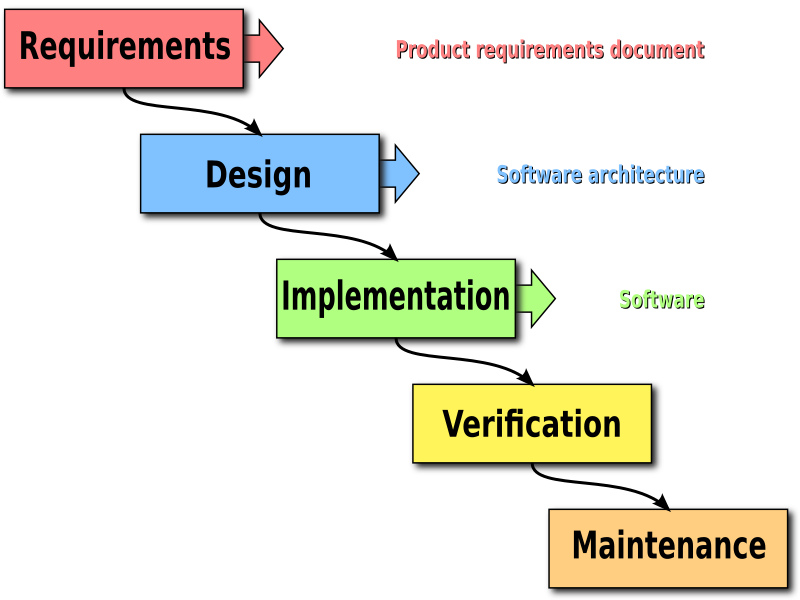
\includegraphics[width=0.6\textwidth,height=0.6\textheight,keepaspectratio]{./img/Waterfall_model.png}
	\caption{Estructura general de una etapa del desarrollo en cascada}
	\label{fig:cascadadesarrollo}
\end{figure}

\section{\textit{Scrum}}

\textit{Scrum} pertenece a las denominadas \textit{metodologías ágiles}, siendo una de las más conocidas \cite{website:scrum}. Su relativa sencillez, así como su flexibilidad y orientación al trabajo en equipo, hace que Scrum sea una de las metodologías más usadas en el desarrollo de software, sobre todo en entornos laborales donde el tamaño del equipo de desarrollo es reducido, aunque su implementación también es posible con equipos mayores, generalmente dividiendo el equipo original en pequeños grupos y manejándolos luego de forma independiente. En la Figura \ref{fig:scrumproceso} se puede observar un ejemplo de cómo funciona \textit{Scrum}.

\subsection{Prácticas recomendadas y bases de \textit{Scrum}}

Uno de los aspectos esenciales de \textit{scrum} es el \textit{sprint}, un bloque temporal (comúnmente de entre 2 y 4 semanas) donde el equipo de desarrollo trabajará para llegar a un objetivo determinado que, generalmente, consiste en acabar todas las tareas definidas para ese \textit{sprint}.
Al principio de cada \textit{sprint} el \textit{product owner}, persona con altos conocimientos sobre el producto que sirve de unión entre el equipo de desarrollo y el resto de la organización, y el \textit{scrum master}, persona encargada de organizar y controlar el \textit{sprint}, junto con el equipo de programadores, definirán lo necesario a realizar en dicho \textit{sprint}. Esto se hará en base a las tareas que se encuentran en el \textit{backlog}, la lista de tareas que se quieren realizar en el producto y que suele ir creciendo a medida que los usuarios encuentran fallos o necesitan nuevas funcionalidades. Normalmente el \textit{product owner} es el encargado de organizar y decidir aquéllas que tienen más prioridad. Todos los integrantes del grupo, así como el propio \textit{product owner} y el \textit{scrum master}, decidirán cuánto esfuerzo o tiempo llevará realizar cada una de ellas, dividiéndola en tareas menores en caso de que sea demasiado grande. También se decidirá qué tareas serán asignadas a cada persona y serán los propios desarrolladores las van eligiendo a medida que finalizan en las que han estado trabajando.\footnote{Algunas compañias llevan Scrum al límite y entrenan a sus empleados para que puedan realizar cualquier tipo de tarea sin limitaciones, por lo que esto es algo que funcionaría muy bien en situaciones similares} De esta manera no todas las tareas tienen un responsable al inicio del \textit{sprint}.
Al principio de cada \textit{sprint} el \textit{product owner}, persona con altos conocimientos sobre el producto que sirve de unión entre el equipo de desarrollo y el resto de la organización, y el \textit{scrum master}, persona encargada de organizar y controlar el \textit{sprint}, junto con el equipo de programadores, definirán lo necesario a realizar en dicho \textit{sprint}. Esto se hará en base a las tareas que se encuentran en el \textit{backlog}, la lista de tareas que se quieren realizar en el producto y que suele ir creciendo a medida que los usuarios encuentran fallos o necesitan nuevas funcionalidades. Normalmente el \textit{product owner} es el encargado de organizar y decidir aquéllas que tienen más prioridad. Todos los integrantes del grupo, así como el propio \textit{product owner} y el \textit{scrum master}, decidirán cuánto esfuerzo o tiempo llevará realizar cada una de ellas, dividiéndola en tareas menores en caso de que sea demasiado grande. También se decidirá qué tareas serán asignadas a cada persona y serán los propios desarrolladores las van eligiendo a medida que finalizan en las que han estado trabajando.\footnote{Algunas compañias llevan Scrum al límite y entrenan a sus empleados para que puedan realizar cualquier tipo de tarea sin limitaciones, por lo que esto es algo que funcionaría muy bien en situaciones similares} De esta manera no todas las tareas tienen un responsable al inicio del \textit{sprint}.

Durante cada día del desarrollo hay una pequeña reunión llamada \textit{sprint stand-up} donde cada uno de los programadores comenta brevemente lo que ha hecho el día anterior, qué tiene planteado realizar ese día y si se ha encontrado con algún problema que le impida continuar.

Al acabar cada \textit{sprint}, el equipo se reúne de nuevo para analizar lo que ha ido bien, qué problemas hubo y las mejoras que deben aplicarse y tenerse en cuenta de cara al futuro, así como elaborar un resumen de estadísticas del equipo. De esta manera, cada nuevo \textit{sprint} será más preciso (dado que sabremos la cantidad de trabajo que el equipo de desarrollo es capaz de hacer en el periodo de tiempo definido) e incluirá el \textit{feedback} de los propios programadores.

Aunque las anteriores son las características esenciales de \textit{Scrum}, al tratarse de una metodología ágil, nada es inamovible y existen bastantes variaciones que se adaptan a todo tipo de equipos tales como la inclusión de otras metodologías. Dependiendo de la empresa, del equipo de trabajo y de las necesidades del mismo, se pueden cambiar o introducir nuevas ideas que mejoren el proceso para ese marco.

\begin{figure}[H]
		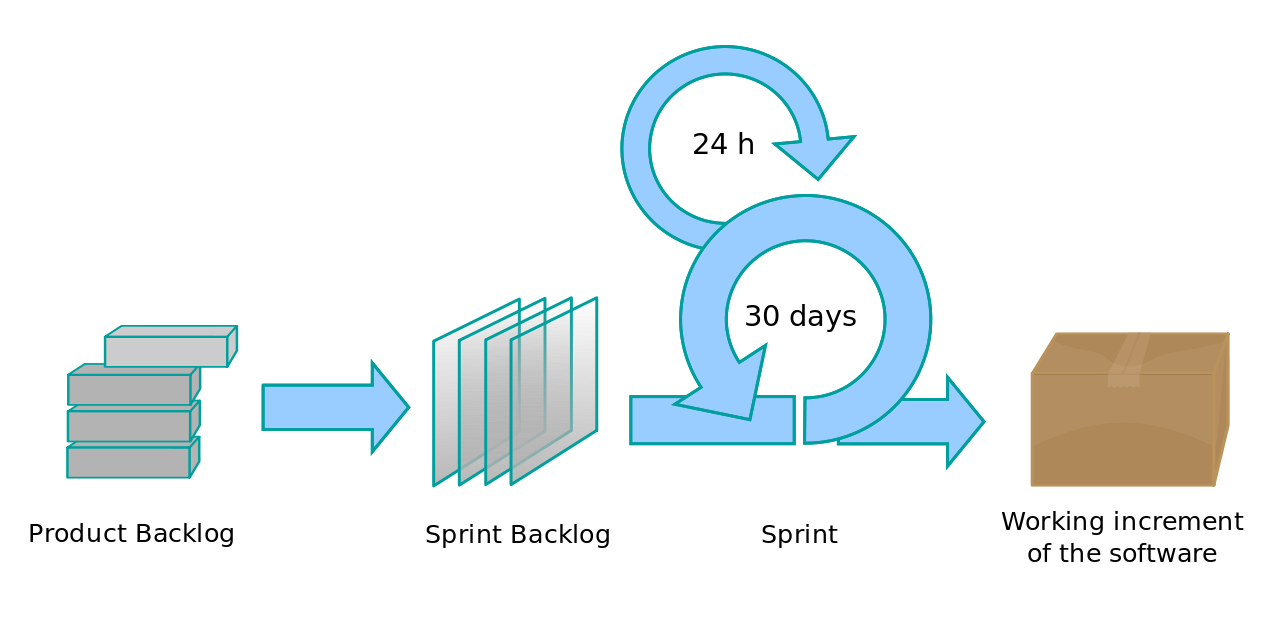
\includegraphics[width=\textwidth,height=\textheight,keepaspectratio]{./img/scrumprocess.png}
	\caption{Proceso concreto de \textit{Scrum} (en este caso el \textit{sprint} dura cuatro semanas)}
	\label{fig:scrumproceso}
\end{figure}

\subsection{Valores}

\textit{Scrum} se basa en flexibilidad y trabajo en equipo. Este es el motivo por el que es muy importante tener un equipo que tenga claro y cumpla con una filosofía y valores básicos. Estos valores son los siguientes:

\begin{itemize}

\item{\textbf{Concentración}} Al tener que finalizar las tareas asignadas antes del final del \textit{sprint}, la concentración del equipo en general y de cada uno de los miembros en particular, es esencial. Para lograr este objetivo, el \textit{product owner} es el encargado de responder las preguntas del resto de la compañía en nombre de los desarrolladores y solamente molestarlos en caso de que sea realmente necesario.

\item{\textbf{Coraje}} Dado que \textit{Scrum} es una metodología de equipo, la ayuda entre cada uno de los miembros es primordial. De igual modo, cada persona debe ser capaz de enfrentarse a nuevos retos y asumir nuevas responsabilidades para que, en su conjunto, el producto final sea el deseado. 

\item{\textbf{Compromiso}} Cada integrante tiene que saber lo que debe hacer y comprometerse a ello. Una vez la reunión inicial haya terminado, es preciso que cada desarrollador sepa en lo que tiene que trabajar, y pregunte al responsable de la tarea en caso de que no tenga algo claro o crea que no puede llegar a terminar lo acordado durante la reunión. Cada programador debe comprometerse con lo establecido para lograr el éxito del equipo.

\item{\textbf{Sinceridad}} Ser capaz de asumir los errores personales y del propio equipo es la clave para mejorar y evolucionar. Si un miembro del equipo de desarrollo se queda estancado en un problema y no avisa al resto de sus compañeros, el \textit{sprint} en su totalidad puede llegar a fracasar por su culpa. Asumir responsabilidades, errores y pedir ayuda cuando sea necesario debe ser una práctica habitual para que esta metodología funcione sin problemas.

\item{\textbf{Respeto}} En la misma línea que el anterior punto, al trabajar en equipo es imprescindible que tanto los logros como los fracasos se tomen como una forma de aprender y mejorar, por lo que el respeto mutuo y asumir los fallos cometidos durante la iteración es la mejor forma de evolucionar, tanto individualmente como en equipo.

\end{itemize}

\section{Metodología elegida}
\label{sec:metodologiaelegida}

Nuestro enfoque ha sido el de partir de una metodología clásica en cascada integrando elementos de \textit{Scrum} y otras metodologías y prácticas relacionadas, tal y como explicamos a continuación.

Para los elementos principales del sistema, tales como la creación de los mapas, enemigos, motor de generación de frases, etc., nos hemos basado en la metodología en cascada para analizar lo que tenemos que realizar, crear el diseño, implementarlo (empezando siempre por los tests, tal y como comentaremos a continuación) y verificarlo. Sin embargo, y dado que los juegos tienden a querer mejorarse continuamente con nuevos elementos de diferente importancia y tamaño (tanto por nuestra parte como por parte de los jugadores-testadores), tiene sentido mantener un \textit{backlog} con todas las nuevas ideas que vayamos recibiendo y el \textit{feedback} recogido, algo para lo que \textit{Scrum} es ideal. 
También hemos tomado la idea de la creación de tareas cortas y \textit{sprints}, de tal forma que en cada una de las iteraciones intentaremos tener un elemento del juego finalizado, siempre y cuando nuestras estimaciones iniciales no se vean comprometidas. De esta manera seremos capaces de seguir más fácilmente el progreso que hemos realizado y tendremos constancia de los nuevos elementos que queremos implementar en un futuro, así como de los \textit{bugs} a arreglar en próximos \textit{sprints}.
Al acabar con el núcleo del juego, la mayor parte de las tareas a realizar a continuación son pequeños cambios y nuevos elementos que no trastocan el diseño inicial del proyecto, por lo que emplear una metodología ágil como \textit{Scrum} es el mejor paso a seguir para terminar las tareas más relevantes lo antes posible. Además, el juego en sí ha sido desarrollado con la idea de hacerlo lo más ampliable y extendible posible. De esta forma, incluso aunque tengamos que cambiar algo en medio del desarrollo, las bases creadas serán sólidas y fácilmente modificables. 

Por último, también hemos seguido la práctica de \textit{test driven development} (desarrollo guiado por pruebas) cuya base consiste en que por cada nueva tarea a realizar, deberemos implementar primero los tests unitarios (que, lógicamente, fallarán en un principio) y luego programar la solución en sí para que el test sea válido, refactorizando la solución en caso de que no sea la ideal. Esto nos dará desde el primer momento una idea clara de lo que queremos hacer antes de proceder con la implementación y nos asegurará de que siempre tendremos el test hecho.